%%% Local Variables: 
%%% mode: latex
%%% TeX-master: "../KanjiHWR"
%%% End: 

\chapter{Conceptual Design of Kanji-Coach}
\label{chap:conceptualdesignofKanjicoach}

\section{Requirements of a Kanji Teaching E-Learning Application}
\label{sec:concept:requirements}

\subsection{General Considerations}
\label{sec:concept:generalconsiderations}

In order to create a concept for a Kanji teaching application,
a number of different aspects need to be taken into consideration.
These aspects emerge from the academic background concerning the Japanese script,
pedagocical and didactic knowledge about teaching languages and general
conceptions of e-learning applications.

Many efforts in designing e-learning applications are focused around the
teacher's view on learning. For designing an e-learning application that
is useful to students, the students view needs be taken into 
account~\shortcite{Alexander2007}. 
\shortciteANP{Ivashin2009}~\citeyear{Ivashin2009} critisises the technical 
dominance in e-learning and e-teaching processes, as the conceptual software
designs are not always supporting the didactic purpose of the software.
Therefore, the user view should be taken into account when conceptually designing
an e-learning application.
The requirement of a \emph{user-focused design} follows directly from this view.

For online e-learning, it is a known that readers only scan the textual 
information displayed. Therefore it is not useful to provide a user with 
large blocks of text, but rather with smaller chunks that encourage 
skimming over~\shortcite{Hamid2001}. It can be expected that the fact
that an e-learning process happens online does not greatly affect the user 
behaviour. Therefore, the observations made for online e-learning can
probably be applied to offline desktop application based e-learning.
The requirement of \emph{keeping textual information short and concise} derives
from the observation.

If e-learning is considered as a learning method in higher education, 
\emph{blended learning} seems to be the most suitable form of e-learning.
That means, combining classroom activities with e-learning 
methods~\shortcite{Hettinger2008,Kahiigi2008}. Language learning is not 
necessarily considered as higher education. In case of studying Japanese,
with its specific difficulties in language and the script, language learning
is taken to an intellectual level that is at least close to higher education.
Therefore, an e-learning application for any aspect of the Japanese language 
should not have the pretensions of posessing the capability 
to \emph{teach Japanese}. Japanese is a complex language with a complex script.
Therefore, e-learning applications should aim at supporting a learner's 
classroom efforts of studying the language. The requirement of 
\emph{focussing on a specific language aspect} can be drawn from this reasoning.
The prototype system designed in this work does not aim at being a complete
system, but rather offers individual learning components from which a user can 
choose what type of learning and which component best supports his study.

\subsection{Classification of a Kanji Teaching Application}
\label{sec:concept:classificationofaKanjiteachingapplication}
%xxx What follows from E-Learning aspects of the whole thing?
%classification as an e-learning application.
%what type of application is it?
%which learning paradigm is followed?

In section~\ref{sec:elearn:classification} different types of e-learning systems
have been discussed. In the course of designing a prototype system, 
design choices need to be made.
The design choice for the prototype will be an offline e-learning system,
that runs on a desktop PC.
This design choice does not follow a conceptual requirement, in fact it ignores
\shortciteANP{Ivashin2009}'s~\citeyear{Ivashin2009} criticism of technical 
dominance in e-learning systems. The choice is a purely technical choice, 
yet, it is driven by a conceptual requirement.
The purpose of the e-learning environment is to test to what extend a handwriting
recognition engine can help studying the Kanji. In order to examine that 
research question, the handwriting recognition needs to be implemented and 
integrated with the e-learning system. 
Thus, the design choice for an offline system was inevitable in the sense that 
the technical limitations of on-line applications form an obstacle for pen 
input of characters and fast recognition procedures.

According to the definition given by~\shortcite{Richert2007} the Kanji teacher 
prototype is a \emph{computer based training} (CBT) system, as it does not use 
the Internet for communication or a webserver for storage. 
According to her research, another criterion for an identifying offline systems 
is that they are offered for distribution on CD-ROM or floppy disk.
That criterion can be regarded as obsolete, as it refers to specific storage 
media. Even if a higher level of abstraction is used to describe the
criterion, it is still obsolete, since \emph{a passive storage medium} is not 
necessary to describe what the criterion actually tries to define.
The criteria concerning communication and data storage are useful to confine
different types of e-learning applications.
Additionally, \emph{installability} can be used as a criterion for offline 
e-learning systems. \emph{Installability} here refers to 
\emph{the possibility to install a software on a computer system}, 
not the \emph{ease of installation}, 
which is defined in ISO9126 as \emph{installability} as 
well~\shortcite{Chua2004}. 
The ISO9126 type of installability will be taken into account during the software
evaluation, which is reported in chapter~\ref{chap:implementationevaluation}.

Concerning the level of interactivity described in 
section~\ref{sec:elearn:interactivity} the prototype designed in this work is 
aimed at a level higher than 
level~\emph{(\ref{elearn:class:changingcontent})~Changing the content of a 
component}. It is targeted between the 
levels~\emph{(\ref{elearn:class:generateobjects})~Generating objects or 
the content of a representation} 
and~\emph{(\ref{elearn:class:constructivemanipulative})~Constructive and 
manipulative actions through situation-dependent feedback}.
Concretely, a user can:
\begin{itemize}
 \item Change the ideal shape of a character by storing a new gold standard.
 \item Create new characters and their descriptions
 \item Receive situation-dependent feedback even on the newly created characters,
       due to the nature of the error recognition algorithm that evaluates
       mathematically the distance between a gold standard character and
       a an input.
       Additionally, characters are analysed structurally, therefore new 
       characters added by the user will automatically be classified and arranged
       among the other characters in the database of the system.
\end{itemize}
Thus, based on the levels of interactivity~\shortcite{Richert2007},
it can be concluded that the prototype provides a very high level of 
interaction. The levels serve as an evaluation measurement for the quality of 
e-learning applications.

\subsection{Conceptual Issues for E-Learning of Kanji}
\label{sec:elearn:conceptualissuesforelearningofKanji}

An e-learning application for Kanji should be an e-learning application for
vocabulary at the same time. It is conceptually not useful to split those two 
learning tasks~\shortcite{Stahlmann2004}.
Learning Kanji and Hànzì is a visual task. Learners need to focus on many little
details concerning a character. For example, the character~\cjk{曜} contains 18 
strokes that are difficult to distinguish from each other in a regular script 
size of 11pt. It is those details that make it difficult for a learner to 
remember a character. Thus, it is important to direct and guide the learner's 
perception of the characters towards a construct of Radicals, rather than a 
combination of a large number of strokes~\shortcite{Stahlmann2004}.
When attempting to split characters into conceptual sub units for the ease of
a learner, two different approaches lend themselves to this goal.

Firstly, splitting the characters into certain strokes. There are 26 original 
strokes in the writing system and each shape in all the characters can be drawn
with a combination of those strokes~\shortcite{Foljanty1984}.
This approach does not seem to ease the task of memorising the Kanji.
It may be fairly easy to memorise 26 strokes, but the fact that around 
2000 Kanji, necessary for reading Japanese, consist of these strokes does not
imply that memorising those becomes any less difficult.

Secondly, splitting the characters into graphemes. There are several shapes
in use in the Japanese and Chinese writing system. There are 79 graphemes in 
use~\shortcite{Hadamitzky1995}.
Using graphemes as a conceptual unit for a learner seems much more useful than
employing the strokes as a direct sub unit of the Kanji.
Memorising all the graphemes may help a learner to study the Kanji, because all 
sub shapes of the characters are known. However, graphemes do not necessarily 
bear a meaning. Therefore, seen from a perspective of perception and cognition, 
the coherence between the different parts of a Kanji would be purely visual.
That can help learners with an outstanding visual memory, but probably not
the majority with an average visual memory.

Thirdly, splitting the characters into Radicals. Radicals are the conceptual 
sub units of Kanji characters and they bear a meaning of their 
own. The number of Radicals is larger than the number of graphemes, but not all 
Radicals are in use and some graphemes are Radicals themselves at the same 
time~\shortcite{Hadamitzky1995}.
The Radicals do not only bear a meaning, but also have a function in character
formation (see section~\ref{sec:typologyoftheKanji} for typology of the Kanji).
In order for a learner to memorise the Kanji, it seems useful to grasp the 
concept of Kanji typology and therefore character formation.
Equipped with the rules of character formation and a number of Radicals the
brain can link different parts of a Kanji character with other parts and 
other characters. For example when studiying phonograms, the majority of the
Kanji characters, knowledge about the pronunciation of the phonetic Radical
will help the learner.

Among those three possibilities it seems most suitable to use a combination of 
the second and the third. Conceptually, the characters will be split into 
Radicals, but the system must know about the concept of a grapheme, too.
Ideally, the system would have data that distinguishes both.

\section{Approaching the Specific Difficulties of the Japanese Script}
\label{sec:concept:tacklingdifficulties}

Section~\ref{sec:japanesedifficulties} deals with the typical problems that 
learners face when studying the Kanji. The Japanese script inevitably bears some 
difficulties when attempting to study it. The application should care for these 
problems by supporting these issues.


\subsection{Character Learning Aspects}
\label{sec:concept:charaterlearningaspects}

The specific problems mentioned in section~\ref{sec:learnersproblems} are:
\begin{enumerate}
  \item \textbf{Similar Kanji} \label{enum:charlearning:similarKanji}
  \item \textbf{Compounds} \label{enum:charlearning:compounds}
  \item \textbf{Unusual readings} \label{enum:charlearning:unusualreadings}
  \item \textbf{Alternative Kanji} \label{enum:charlearning:alternativeKanji}
  \item \textbf{Homophones} \label{enum:charlearning:homophones}
  \item \textbf{Infrequent Jōyō Kanji} \label{enum:charlearning:infrequenjoyo}
  \item \textbf{Non-Jōyō Kanji} \label{enum:charlearning:nonjoyo}
\end{enumerate}

\subsubsection{Problems Outside the Scope of the Prototype}
\label{sec:concept:problemsoutsidescope}

A Kanji teaching prototype cannot provide solutions for all of those problems,
but for some. It cannot provide a satisfying solution for 
problem~\ref{enum:charlearning:compounds} as the prototype deals with single
characters only. It is not useful to provide a solution for 
problem~\ref{enum:charlearning:unusualreadings} because studying the main
reading of a character is most important at the beginning. Especially, when
studying a new character, the learner should focus on the character shape and
the main reading, not on unsusual alternative readings. Kanji Coach aims
at teaching the Japanese script, not the full Japanese language.

Kanji Coach cannot provide a solution for 
problems~\ref{enum:charlearning:infrequenjoyo} 
and~\ref{enum:charlearning:nonjoyo}, memorising infrequent Jōyō 
Kanji and Non-Jōyō Kanji. These characters are difficult because they are 
infrequent. It seems more suitable for a learner to study the frequent characters
first in order to learn reading and writing. Thus, it is not plausible to pay 
special attention to this group of characters by presenting those moreoften to 
the learner.

\subsubsection{Problems Inside the Scope of the Prototype}
\label{sec:concept:problemsinscope}

The two main problems for learners of Japanese Kanji are 
\begin{itemize}
  \item Similar Kanji (problem~\ref{enum:charlearning:similarKanji})
  \item Homophones (problem~\ref{enum:charlearning:homophones})
\end{itemize}
Those two will be dealt with in the prototype. Additionally, the problem of
\begin{itemize}
  \item Alternative Kanji (problem~\ref{enum:charlearning:alternativeKanji})
\end{itemize}
is targeted by the e-learning application.

\paragraph{Similar Kanji} are the major issue for a learner of Japanese. The 
prototype \emph{Kanji Coach} provides a solution for this difficulty.
The solution does not necessarily contain the employment of specialised lessons 
for similar-looking Kanji. The reason for that is that it is more suitable for 
the human brain to study material that belongs to the same range of topics. 
Similar looking Kanji often do not have a connection to each other except their 
visual similarity. Therfore, studying them together does not seem useful,
unless they are semantically similar, too, like for instance the characters for
\emph{speaking} \cjk{話}, \emph{state/give instructions} \cjk{誥} and 
\emph{language} \cjk{語} that also belong to the same Kanji class, 
as their key Radical is the same.

\paragraph{Homophones} are a general difficulty for learnears of the Japanese 
language. Many words are phonetically ambiguous. The context can provide a better
understanding, but often it is necessary to see the written Kanji character in 
order to know what is meant with an expression~\shortcite{Foljanty1984}.
Therefore, it is essential to deal with 
problem~\ref{enum:charlearning:homophones}. 

Conceptually, this issue can be solved by providing special lessons that focus on
homonphones. Homophones in Japanese are not necessarily homographs and therefore 
not homonyms in the strict sense. True homonyms are those word pairs that are 
both homophones and homographs. In languages using Latin characters,
homophones are often homographs at the same time, e.g.\ German \emph{Schloss} 
(Eng.\ castle) and \emph{Schloss} (Eng.\ lock). This is due to the fact that
the spelling roughly mimics the speech. The pairs that are both homophones and
homographs are called homonyms. Sometimes, homophones are not homographs, 
e.g.\ the verbs \emph{dye} and \emph{die}.

In the course of studying the Kanji, it is part of the study process to 
learn to distinguish the characters that are pronounced the same.
For instance, there are roughly 80 distinct characters that share the
pronounciation \emph{kyo}. Table~\ref{table:kicombinations} on 
page~\pageref{table:kicombinations} shows several Kanji that are 
pronounced~\emph{ki}. The prototype provides a lesson that is centred around 
the homophone Kanji characters and their distinction.

\paragraph{Alternative Kanji} is an issue that can be dealt with in an indirect
way. Following the concept that frequent characters and the main reading should 
be studied first, Kanji Coach does not provide any special form of presentation
for this group of characters. However, it has the ability to recognise 
alternative Kanji. In a scenario where a user is asked to input a certain 
character, an alternative character with the same meaning would be accepted. 
For instance, if a user is promped for the character for the number \emph{one}, 
which is usually written as~\cjk{一}, but enters the character~\cjk{壱} instead
this input would be regarded as correct. Additionally, the user is presented 
with a hint that another character with the same meaning exits. 
The focus lies on studying the frequent characters, therefore there are no 
special lessons concerning alternative Kanji.

\subsubsection{Character Repetition}
\label{sec:concept:characterrepetition} %label in use already.

In section~\ref{sec:elearn:elearningoflanguages} the pure repetition of 
grammatical structures as a learning method has been critisised.
The system should account for that by not just forcing the user to
reproduce fixed structures. In fact, it should leave room for creativity.
The system does not provide a free-drawing module in order to allow for
total creativity. But, creativity is given through the use of the
Handwriting input as such. A user can practice his own writing style.
The tolerance thresholds given by the character recognition allow for a
interpretation of the character shape, rather than a pure repetition.

%Zum Beispiel - radikale vorgeben und zeichen schreiben lassen.
%und ganz generell: toleranzgrenzen erlauben kreativitaet allein schon deswegen,
%weil selbst der zeichenstift benutzt wird.

\section{Integration of HWR Into the Learning Process}
\label{sec:concept:integrationofhwrintolearning}

The learning process of Kanji is driven by understanding the structre and 
meaning of the characters and memorising the shape~\shortcite{Stahlmann2004}. 
In order to study and memorise, many learners rely on repeating to write the 
Kanji. That approach seem most natural and can hardly be replaced by anything.

\subsection{The Motivation for Using a HWR}
\label{sec:concept:motivationforusinghwr}

The fact that learning to read and learning to write is an intervowen process 
suggests that both should be studied together. In standard class room learning 
environments that is the case. Learners read texts, are presented with new
Kanji and are asked to reproduce the Kanji when writing essays.
An e-learning application can not perform the teaching effort of a full language
course. In order to provide complementary addition to a language course,
the prototype should create an environment that increases the user's regalement 
for tedious learning tasks.

The repetition of writing characters in order to memorise them does not
appeal to the majority of the learners. Especially having to write on paper
repeating the same character over and over again does not awake inspiration
and creativity. An e-learning application with an integrated handwriting 
recognition engine that provides corrections for the user inupt has two 
main functions:
\begin{itemize}
  \item Making the repetitive task of training the muscular memory less tedious.
  \item Helping the learner overcome difficulties in writing the Kanji by 
        giving informed feedback.
\end{itemize}
In order to train the muscular memory and memorise the Kanji, repetition is 
needed. The same amount of written characters can seem less repeating simply if
the characters are not written in a row. Additionally, using a technical device 
can be more emotive and help increasing the user's motivation and 
self-discipline. \shortcite{Ismail2002,Richert2007} critised that some 
e-learning applications do not add a value to the learning 
process.\footnote{For details see section~\ref{sec:elearn:elearningoflanguages}.}
Additional value over practising to write characters on paper is added
by the following features:
\begin{itemize}
  \item The general possibilities of the application to prompt the user with 
        different characters
  \item Presenting new characters, their meanings, pronunciation and
        stroke order.
  \item Having the characters organised in lessons and teaching related
        characters in combination.
  \item The different methods
    \begin{itemize}
      \item Writing a Japanese character after being prompted an English word, 
            instead of purely drawing lines without an additional cognitive 
            anchor.
      \item Writing a Japanese character after being prompted a Japanese word.
    \end{itemize}
  \item The error correction that comes with the handwriting recognition. The 
        user is less dependend on a teacher and can study in his own time and 
        pace, yet still get informed feedback.
\end{itemize}
 
\subsection{Character Recognition}
\label{sec:concept:characterrecognition}

The type of character recognition is crucial for the abilities of the system 
concerning error processing. Highly optimised handwriting recognition systems
perform a fast and reliable handwriting recognition. However, those systems
often do not have a  record of the internal structure of the 
characters.\footnote{See chapter~\ref{chap:onlinehwr} for details.}
Since understanding of the structure of the characters is important for a 
successful learning process, the error correction needs to focus on the internal
structure of the Kanji characters. Studying the character shapes can be 
performed as a purely visual task. Studying the full characters and grasping
their construction is a cognitive task that combines visual memory with
linguistic information. Thus, the error correction must provide structural
error levels, considering the internal character structure. Following that
concept even further, the character analysis must be structural, too.
The prototype performs a strucutral character 
recognition.\footnote{The technical details of the character recognition
are described in chapter~\ref{chap:handwritingrecognitionengine}.}

%xxx How do the HWR and the learning process interplay conceptually?
%xxx In what form do the corrections come up?
%xxx What kind of error recognition is there?
%xxx character input: timeout for learning - no button in handwriting data input view

% Wichtige Fragestellung: Wie sieht eine HWR in Lernumgebung aus?
% Mappe S. 19
% genaue anforderungen s. 19!
% waehle bestimmte architekture unter moeglichen ansaetzen.


% welche art von character recognition muss geleistet werden?

% was sind die moeglichkeiten (im vergleich zu anderen produkten),
% die sich durch eine HWR ergeben?
% wie kann man die ausschoepfen? s. 16 unten und s. 15

% Error Recognition
% what type of errors?
% semantical errors? cow vs sheep vs pig
% phonological errors (readings) Kanji that sound the same.
% theoretically: compounds - for the Kanji readings.
% heft: s. 52

% - compare with normal paper-based learning of Kanji
% - compare with other Kanji-learning systems
% klare abgrenzung von skritter.
% s. 51 unten im heft.


\section{Handling Errors}
\label{sec:concept:handlingerrors}

%xxx why this section? what is its purpose?
%because it is one of the crucial novelties of the system to provide an
%error handling like this, therefore it must be reported.

%what is in this section:
%how to deal with errors conceptually
%what types of errors are there and how they can be handled
%outcome visioning: educational aspects / the e-learning view
%how? how will it be structured?
%next action - what to write first?

\subsection{Motivation for Error Recognition}
\label{sec:concept:motivationforerrorrecognition}


\subsection[Sources of Error]{Possible Sources of Error When Writing Japanese Characters}
\label{sec:concept:sourcesoferror}

error handling, see page 58.


See notes on paper, seite 58
- for example stroke number and stroke sequence
- length of strokes

- stroke velocity

\section{Use Cases}
\label{sec:concept:usecases}

Figure~\ref{fig:startupScreen}
\begin{figure}[htbp]
\begin{center}
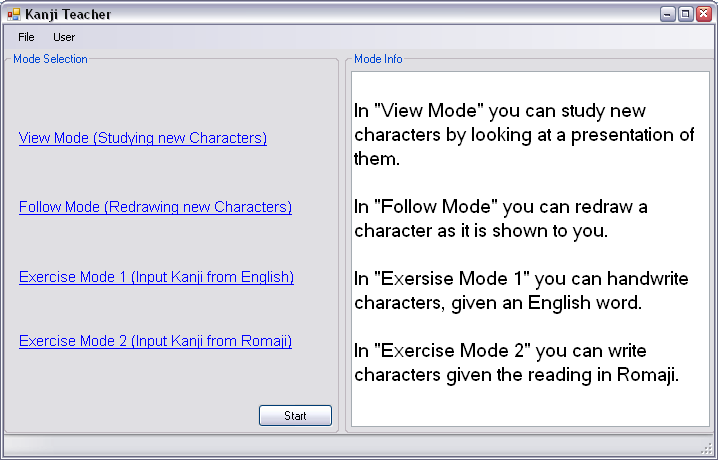
\includegraphics[scale=0.7]{images/ConceptualDesign/startupScreen.png}
\caption{Startup screen}
\label{fig:startupScreen}
\end{center}
\end{figure}

Figure~\ref{fig:viewMode}
\begin{figure}[htbp]
\begin{center}
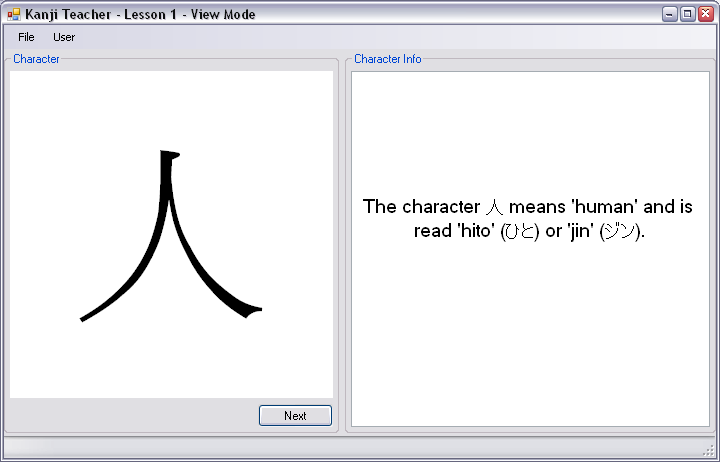
\includegraphics[scale=0.7]{images/ConceptualDesign/viewMode.png}
\caption{Startup screen}
\label{fig:viewMode}
\end{center}
\end{figure}

Figure~\ref{fig:mobileDeviceInput}
\begin{figure}[htbp]
\begin{center}
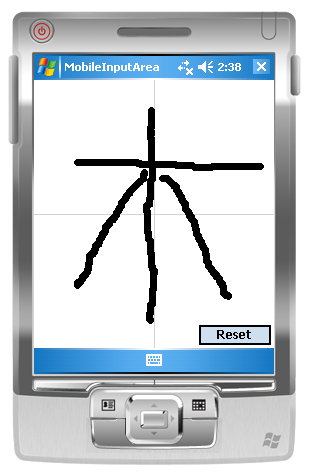
\includegraphics[scale=0.7]{images/ConceptualDesign/mobileDeviceInput.png}
\caption{Startup screen}
\label{fig:mobileDeviceInput}
\end{center}
\end{figure}



% siehe 'screenshot' - grafiken von s. 2 - 9
% auch: was kann man aus e-learning machen?
% welche (technischen) moeglichkeiten sind eroeffnet,
% insbesondere auch durch handschriftenerkennung?

% idee: schoenschreibekurs, bei dem einzelne striche
% gesondert geuebt werden.

